\documentclass[conference]{IEEEtran}
\IEEEoverridecommandlockouts

\usepackage{cite}
\usepackage{amsmath,amssymb,amsfonts}
\usepackage{algorithmic}
\usepackage{graphicx}
\usepackage{textcomp}
\usepackage{xcolor}
\usepackage{booktabs}
\usepackage{array}
\usepackage{multirow}
\usepackage{url}
\usepackage[colorlinks=false, pdfborder={0 0 0}]{hyperref}
\usepackage[normalem]{ulem}

\def\BibTeX{{\rm B\kern-.05em{\sc i\kern-.025em b}\kern-.08em
    T\kern-.1667em\lower.7ex\hbox{E}\kern-.125emX}}

\let\OLDthebibliography\thebibliography
\renewcommand\thebibliography[1]{
  \OLDthebibliography{#1}
  \setlength{\itemsep}{0pt}
  \setlength{\parskip}{0pt}
}

\begin{document}

\title{ A Compliance Scoring Framework for XAI in High-Risk Credit Scoring: Evaluating SHAP and LIME Against EU AI Act Articles 13, 14, and 26}

\author{
\IEEEauthorblockN{Samrat Lamsal}
\IEEEauthorblockA{\textit{School of Computer Engineering} \\
\textit{KIIT Deemed to be University} \\
Bhubaneswar, India \\
lamsalsamrat831@gmail.com}
\and
\IEEEauthorblockN{Sumana De}
\IEEEauthorblockA{\textit{School of Computer Engineering} \\
\textit{KIIT Deemed to be University} \\
Bhubaneswar, India \\
sumana.defcs@kiit.ac.in}
\and
\IEEEauthorblockN{Sulav Poudel}
\IEEEauthorblockA{\textit{School of Computer Engineering} \\
\textit{KIIT Deemed to be University} \\
Bhubaneswar, India \\
sulavpoudel44@gmail.com}
}

\maketitle

\begin{abstract}
The EU Artificial Intelligence Act (Regulation 2024/1689), enforceable from August 2, 2026, designates credit scoring as high-risk under Annex III, Category 5(b), imposing legally binding obligations of transparency, explainability, and human oversight. Despite widespread institutional adoption of SHAP and LIME, no prior framework systematically maps XAI method properties to specific statutory requirements. This paper introduces the Compliance Scoring Framework (CSF): seven operationalized criteria derived directly from Articles 13, 14, and 26, each with an explicit measurement method and a literature-grounded score conversion. These scores reflect how well each method supports regulatory objectives — they are not a finding of legal compliance. We apply the CSF to SHAP and LIME explanations generated by a LightGBM classifier on 307,511 real credit applications (Home Credit, 2018). The most consequential differentiators are explanation consistency (Jaccard: 1.000 vs. 0.381; paired Wilcoxon $W=0$, $p<10^{-17}$), bias detection sensitivity (gender present in 100\% of SHAP explanations vs. absent from LIME's top-10 in 92.5\% of instances), and auditability infras- tructure burden; SHAP's overall compliance score is 4.12/5.00 versus LIME’s 2.50/5.00. A kernel width sensitivity sweep across a 12× range confirms LIME’s low fidelity ($R^2 = 0.251$) is a structural property of the model–dataset combination, not a configuration artifact. LIME demonstrates a meaningful advantage in user comprehensibility (4.0 vs. 2.0). We propose a hybrid deployment strategy and document seven limitations transparently.

\end{abstract}

\begin{IEEEkeywords}
Explainable AI, EU AI Act Compliance, Credit Scoring, SHAP, LIME, LightGBM, Regulatory Framework, Fairness, Auditability
\end{IEEEkeywords}

\section{Introduction}

Explainability of AI-driven credit decisions is not merely
a technical aspiration but an emerging legal requirement. The
EU Artificial Intelligence Act (Regulation 2024/1689) \cite{b2}, in
force August 2024, classifies automated credit scoring as high-risk
under Annex III, Category 5(b), with full compliance obligations
from August 2, 2026. Non-compliance risks fines of up to
\texteuro{}35 million or 7\% of global annual turnover, transforming Explainable Artificial Intelligence
(XAI) method selection into a regulatory decision.

Articles 13, 14, and 26 bear most directly on explainability. Article 13 requires transparency sufficient to ``correctly interpret'' system output; Article 14 mandates human oversight enabling detection of biased outputs; Article 26 imposes parallel deployer monitoring obligations \cite{b2,b3}.

SHapley Additive exPlanations (SHAP) \cite{b4} and Local Interpretable Model-agnostic ExplanationS (LIME) \cite{b5} dominate financial XAI practice, yet comparative literature evaluates them on technical dimensions without grounding criteria in statutory text \cite{b8,b9}. Without a compliance-oriented framework, institutions cannot determine which method satisfies their legal obligations. A method producing inconsistent explanations may be misaligned with Article 13(3)(b); one that fails to surface demographic attribution gaps may be structurally limited under Article 14(4)(b). This gap is acute given the August 2026 deadline and the absence of EU AI Office implementation guidelines.

This paper contributes: (1) the CSF---seven criteria derived from Articles 13, 14, and 26 with operationalized metrics and literature-grounded thresholds; (2) empirical evaluation on 307,511 credit applications including a kernel width sensitivity sweep and fixed-seed consistency analysis; and (3) a hybrid deployment strategy grounded in per-article regulatory requirements.

\section{Related Work}

Hacker and Eber~\cite{b3} analyse credit underwriting under the Act,
finding that Articles 13 and 14 impose obligations exceeding current
banking law. Lundberg and Lee~\cite{b4} established SHAP's
Shapley value foundation. Ribeiro et al.~\cite{b5}
introduced LIME as a model-agnostic local approximation via perturbed
samples. Guidotti et al.~\cite{b8}
provide a taxonomy of black-box explanation methods. Nauta et
al.~\cite{b9} review XAI evaluation criteria across
correctness, completeness, and consistency dimensions. Subsequent work
formalised TreeSHAP~\cite{b11} for exact computation on
tree models. Both SHAP and LIME have been applied in credit
scoring~\cite{b15}.

Kaur et al.~\cite{b6} show that practitioners frequently
misinterpret XAI outputs, establishing that semantic accessibility
matters beyond technical fidelity. Alvarez-Melis and
Jaakkola~\cite{b14} formalise local explanation robustness, providing
theoretical grounding for Jaccard-based consistency evaluation.
Panigutti et al.~\cite{b7} conduct an interdisciplinary analysis of XAI
in the context of the AI Act, focusing on Articles 13 and 14, arguing
that its obligations are functional rather than methodological---it does
not mandate specific XAI methods, leaving an operationalization gap. To
our knowledge, no prior work operationalizes selected requirements of
the EU AI Act as measurable and reproducible criteria for evaluating
XAI methods---the gap this paper addresses.

\section{Methodology}

\subsection{Dataset, Preprocessing, and Model Selection}

We use the Home Credit Default Risk dataset~\cite{b10}: 307,511 loan
applications with 122 features spanning applicant demographics,
financial history, credit bureau data, and loan characteristics. The
binary target variable encodes default (positive class, 8.1\%) versus
full repayment (91.9\%). Preprocessing: missing values imputed using
column medians; categorical variables label-encoded; columns with
100\% missing values excluded (none were present), retaining 120
features. A stratified 64/16/20 split produces training (196,806),
validation (49,202), and held-out test (61,503) sets. For all
three architectures, we kept hyperparameters at values standard in the
literature and did no architecture-specific tuning. The one exception
was LightGBM's number of boosting rounds, which was set by early
stopping on the validation set. Table~I reports the outcome of that
comparison --- and because the test set was used only at that point,
it also stands as the final performance report for the chosen model.

Three classifiers were compared: Logistic Regression (AUC-ROC: 0.619),
Random Forest (0.733), and LightGBM~\cite{b1} (0.759). LightGBM was
selected for highest predictive performance and native TreeSHAP
compatibility~\cite{b11}, which enables exact Shapley value computation
without Monte Carlo sampling.

\begin{table}[h]
\caption{Model Performance Comparison (Test Set, $n = 61{,}503$)}
\label{tab:model_perf}
\centering
\begin{tabular}{lcccc}
\toprule
\textbf{Model} & \textbf{AUC-ROC} & \textbf{Precision} & \textbf{Recall} & \textbf{F1} \\
\midrule
Logistic Regression & 0.619 & 0.111 & 0.576 & 0.186 \\
Random Forest       & 0.733 & 0.169 & 0.594 & 0.263 \\
LightGBM $\bigstar$ & 0.759 & 0.170 & 0.679 & 0.272 \\
\bottomrule
\multicolumn{5}{l}{\footnotesize $\bigstar$ Selected for XAI analysis. All metrics on held-out test set only.}
\end{tabular}
\end{table}

\subsection{XAI Configuration}

SHAP values are computed via TreeSHAP \cite{b11} on 1,000 test instances (\texttt{random\_state=42}); top-10 features per instance used for coverage. LIME explanations use 1,000 perturbation samples and 10 features per explanation on the same 1,000 instances. Consistency testing: 100 instances across 10 independent runs; fixed-seed testing fixes \texttt{random\_state=42} throughout.

\subsection{Compliance Scoring Framework: Criteria and Formulas}

The CSF comprises seven criteria (Table~\ref{tab:csf_criteria}) mapped to specific EU AI Act articles, each scored 1--5, where 1 means the method barely satisfies what the article requires and 5 means it does so reliably and completely, against literature-grounded thresholds (Table~\ref{tab:score_thresh}). A high score means the method's technical properties match what the Act appears to require --- it does not mean the institution deploying that method is legally compliant. Quantitative criteria (C1, C2, C3a, C4, C5) are computed automatically; qualitative criteria (C3b, C6, C7) are assessed via structured checklists.

\begin{table}[h]
\caption{CSF Criteria Definitions}
\label{tab:csf_criteria}
\centering
\renewcommand{\arraystretch}{1.2}
\begin{tabular}{p{0.28cm}p{2.0cm}p{1.4cm}p{0.7cm}p{1.5cm}}
\toprule
\textbf{ID} & \textbf{Criterion} & \textbf{EU AI Act Article} & \textbf{Type} & \textbf{Metric} \\
\midrule
C1  & Attribution Coverage / Fidelity     & Art. 13(1)   & Quant.  & Coverage \% / $R^2$ \\
C2  & Explanation Consistency             & Art. 13(3)(b)& Quant.  & Jaccard $J$ \\
C3a & Structural Complexity               & Art. 13(1)   & Quant.  & SC index \\
C3b & User Comprehensibility              & Art. 13(1)   & Qual.   & Checklist \\
C4  & Bias Detection Capability           & Art. 14(4)(b)& Semi-Q. & $|\bar{\varphi}_2 - \bar{\varphi}_1|$ \\
C5  & Fairness Transparency               & Art. 26(5)   & Quant.  & $|AR_2 - AR_1|$ \\
C6  & Human Oversight Support             & Art. 14(1)   & Qual.   & Checklist \\
C7  & Auditability                        & Art. 13(3)   & Qual.   & Checklist \\
\bottomrule
\end{tabular}
\end{table}

\noindent\textbf{C1 (Coverage / Fidelity):} For SHAP, attribution coverage of top-$k$ features:
\begin{equation}
    C = \frac{\sum_{i \in \text{top-10}} |\varphi_i|}{\sum_{j \in \text{all}} |\varphi_j|}
\end{equation}
For LIME, local surrogate fidelity $R^2$ between surrogate predictions and black-box predictions on the perturbed neighbourhood. The two metrics are not the same thing --- SHAP's coverage is a proportion of total attribution mass, LIME's is a regression $R^2$. But both answer the same underlying question: how much of what the model actually did does this explanation account for? We calibrated the scoring bands separately for each, so a score of 3 means roughly the same thing in practical terms whichever metric produced it.
\smallskip

\noindent\textbf{C2 (Consistency):} Mean pairwise Jaccard similarity
\begin{equation}
    J(S_i, S_j) = \frac{|S_i \cap S_j|}{|S_i \cup S_j|}
\end{equation}
 across all pairs of runs on the same instances. Grounded in
Article~13(3)(b), under which reproducible explanation records
are a functional requirement for reliable audit logging.
\smallskip

\noindent\textbf{C3a (Structural Complexity):}
\begin{equation}
    \text{SC} = 0.4 \cdot \frac{F}{10} + 0.4 \cdot \frac{N_C}{10} + 0.2 \cdot \frac{\bar{L}}{20}
\end{equation}
where $F$ = features in explanation (always $K = 10$), $N_C$ = conditional operators, $\bar{L}$ = mean feature name length; the weights are heuristic and not independently validated against human ratings.
\smallskip


\noindent\textbf{C4 (Bias Detection):} $\Delta = |\bar{\varphi}_1 - \bar{\varphi}_2|$ using signed means per group. Signed rather than absolute attribution values are used to preserve
directional information. Mapped to the bias monitoring objectives of
Article~14(4)(b).
\smallskip

\begin{table}[h]
\caption{Operational Mapping from EU AI Act Articles to Measurable CSF Criteria}
\label{tab:op_mapping}
\centering
\small
\renewcommand{\arraystretch}{1.4}
\begin{tabular}{p{1.6cm}p{1.8cm}p{2.4cm}p{1.4cm}}
\hline
\textbf{EU AI Act Provision} & \textbf{Legal Objective} & \textbf{Technical Requirement (Interpretive Step)} & \textbf{CSF Criterion} \\
\hline
\hline
Art.~13(3) -- Logging \& traceability & Enable auditability and reconstruction of system behavior & Explanation outputs must be reproducible for reliable logging & C2 (Consistency), C7 (Auditability) \\[6pt]
Art.~14(4)(b) -- Identify biased outputs & Enable detection of discriminatory system behavior & Demographic influence must be observable in explanation outputs & C4 (Bias Detection Capability) \\[6pt]
Art.~26(5) -- Deployer monitoring & Enable portfolio-level oversight & System-level disparity metrics must be measurable & C5 (Fairness Transparency) \\
\hline
\end{tabular}
\end{table}


\noindent\textit{Operational Interpretation of Statutory Language.} Table~\ref{tab:op_mapping} maps statutory obligations to measurable criteria. Table~\ref{tab:csf_criteria} follows the same logic. C1, C3a, and C3b all trace back to Article~13(1)'s phrase ``correctly interpret'' --- we read that as requiring that explanations cover enough of the prediction, avoid unnecessary structural clutter, and be readable by non-specialists. C6 connects to Article~14(1): an overseer needs to see which direction a feature pushes the outcome, how strongly, and where in the model that influence originates. These are our readings of broadly worded statutory language; other readings are possible, and we flag this in Section~V-D.
\smallskip

\noindent\textbf{C5 (Fairness Transparency):} Approval rate disparity $|AR_1 - AR_2|$. The CSF does not define binding legal standards; it identifies reproducible technical properties supporting the
functional objectives of Articles 13, 14, and 26. Alternative
operationalizations exist—for example, Article~14(4)(b) could
use counterfactual fairness metrics—and independent legal review
should refine these mappings as regulatory guidance evolves.

\begin{table}[h]
\caption{Score Conversion Thresholds}
\label{tab:score_thresh}
\centering
\renewcommand{\arraystretch}{1.2}
\resizebox{\columnwidth}{!}{%
\begin{tabular}{cccccc}
\toprule
\textbf{Score} & \textbf{Coverage (SHAP)} & \textbf{Fidelity $R^2$ (LIME)} & \textbf{Jaccard $J$} & \textbf{SC (inv.)} & \textbf{Bias Gap $\Delta$} \\
\midrule
5 (Full) & $\geq$90.0\% & $\geq$0.85 & $\geq$0.95 & $\leq$0.40 & $\geq$0.050 \\
4        & $\geq$80.0\% & $\geq$0.75 & $\geq$0.85 & $\leq$0.55 & $\geq$0.030 \\
3        & $\geq$70.0\% & $\geq$0.65 & $\geq$0.75 & $\leq$0.70 & $\geq$0.010 \\
2        & $\geq$60.0\% & $\geq$0.55 & $\geq$0.60 & $\leq$0.85 & $\geq$0.005 \\
1 (None) & $<$60.0\%    & $<$0.55    & $<$0.60    & $>$0.85    & $<$0.005   \\
\bottomrule
\end{tabular}}
\parbox{\columnwidth}{\footnotesize Thresholds: Coverage motivated by Miller \cite{b12} ($k$=10 ceiling, 60\% floor from observed distribution). Jaccard: Alvarez-Melis \& Jaakkola \cite{b14} robustness criteria. Bias gap: disparate impact conventions. Institutions must recalibrate thresholds for their specific architecture and dataset.}
\end{table}

\section{Experimental Results}

\subsection{C1 --- Attribution Coverage and Local Fidelity}

SHAP achieves a mean attribution coverage of $0.700 \pm 0.062$: the top-10 features account for $70.0\%$ of total prediction attribution, scoring $3.0/5.0$. This indicates meaningful coverage but also that substantial attribution mass resides in features ranked 11--120, relevant for institutions performing full attribution logging.

LIME achieves a mean $R^2 = 0.251 \pm 0.136$. A kernel width sensitivity sweep across seven multipliers ($0.25\times$--$3.0\times$, $n = 200$ per configuration; Fig.~1) shows $R^2$ remains flat at $0.2553$--$0.2790$, establishing low fidelity as a structural property of fitting a linear surrogate to a 120-feature gradient boosting model---no kernel width adjustment can resolve the fundamental mismatch between linear and nonlinear decision boundaries. Score: $1.5/5.0$.

We ran the same kind of sweep for three other parameters: perturbation sample size, feature count $K$, and whether discretization was enabled ($n=150$ per configuration). $R^2$ barely moved under either of the first two --- it held in the $0.24$--$0.31$ range across all conditions. Gender's rate of appearing in the top-$K$ list was more sensitive: it spanned 5.3\%--16.0\% across sample sizes, and jumped from 10.7\% at $K=10$ to 76.0\% at $K=20$. The most striking result came from turning off discretization --- fidelity roughly doubled ($R^2=0.248\to0.521$) and structural complexity dropped close to SHAP's level ($\text{SC}=1.044\to0.542$). So some of LIME's poor C1 and C3a performance is specific to how we configured it, not a fixed property of the method --- we document this as Limitation 7.

\begin{figure}[h]
    \centering
    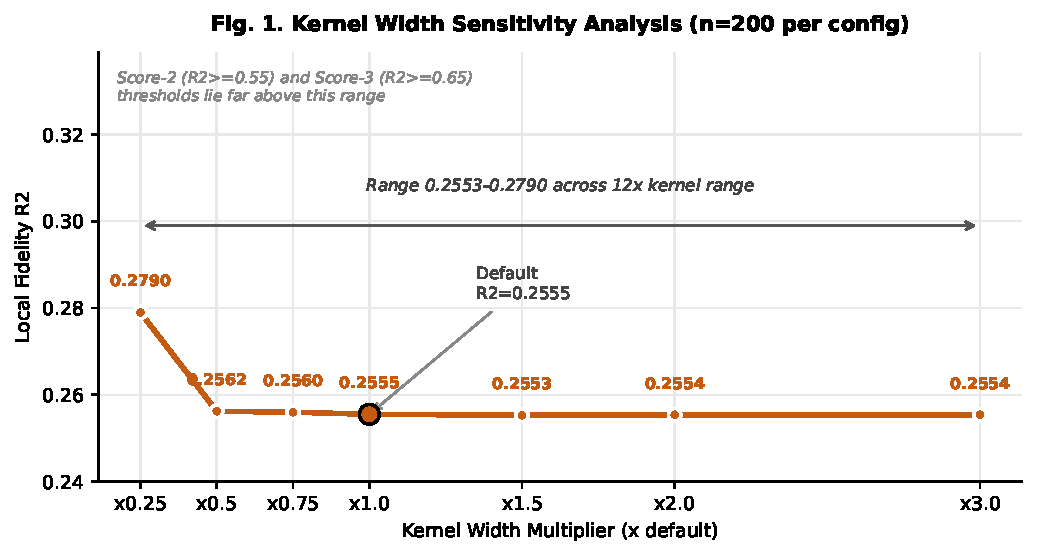
\includegraphics[width=\columnwidth]{fig1_kernel_sweep.pdf}
    \caption{Kernel width sensitivity analysis. $R^2$ range: 0.2553--0.2790 across a 12$\times$ kernel width range ($n$=200 per configuration), establishing low fidelity as a structural property.}
    \label{fig:kernel}
\end{figure}

\subsection{C2 --- Explanation Consistency (Most Critical Finding)}

SHAP achieves $J = 1.000$ ($\pm$0.000), confirming mathematical
determinism. LIME achieves $J = 0.381$ ($\pm$0.114) under
stochastic conditions---only 38.1\% average feature overlap
across runs (Mann-Whitney $U = 20{,}250{,}000$, $p < 0.001$;
Fig.~2). Fixed-seed LIME recovers $J = 1.000$ but requires
per-instance seed storage absent from SHAP's determinism. We should note that those 4,500 pairwise scores are not independent --- the same instances and runs appear in multiple pairs, which could inflate apparent significance. To address this, we aggregated each instance's Jaccard scores across runs (giving one value per instance, $n=100$) and ran a paired Wilcoxon test on those. SHAP came out ahead in all 100 cases without exception ($W=0$, $p<10^{-17}$).

Under Article 13(3)(b) logging objectives, reproducible explanations are a functional requirement. Stochastic LIME shares fewer than 40\% of top features across runs; a denied applicant could receive materially different explanations at different times, creating regulatory exposure. SHAP: 5.0/5.0. LIME: 1.0/5.0.

\begin{figure}[h]
    \centering
    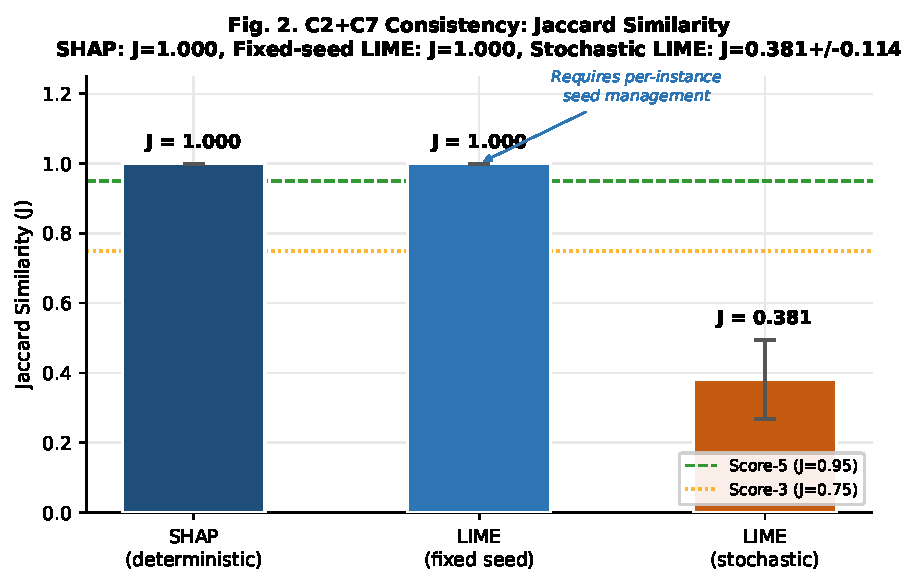
\includegraphics[width=\columnwidth]{fig2_consistency.pdf}
    \caption{C2+C7: Jaccard consistency. SHAP and fixed-seed LIME achieve $J$=1.000; stochastic LIME achieves $J$=0.381$\pm$0.114 ($p$$<$0.001 vs. SHAP). Fixed-seed parity requires per-instance seed management infrastructure.}
    \label{fig:jaccard}
\end{figure}

\subsection{C3 --- Structural Complexity and User Comprehensibility}

SHAP achieves structural complexity $\text{SC} = 0.536 \pm 0.011$, scoring $4.0/5.0$. LIME achieves $\text{SC} = 1.044 \pm 0.010$, exceeding the acceptable threshold of $0.70$. LIME's higher complexity arises from discretization: the surrogate expresses features as conditions (e.g., \texttt{Annual\_Income} $\leq 45{,}000$) that are structurally more complex than a scalar attribution. LIME: $1.0/5.0$.

For user comprehensibility (C3b), the direction reverses.
LIME's condition-based format (`Debt Ratio $>$ 35\%: $-$0.25')
is more interpretable to non-expert users than raw Shapley
magnitudes~\cite{b6}. SHAP: 2.0/5.0. LIME: 4.0/5.0---LIME's
primary and most reproducible advantage.

\subsection{C4 --- Bias Detection Capability}

This criterion exposes a fundamental architectural asymmetry: TreeSHAP computes attributions for every feature unconditionally; LIME's sparse local models miss features not consistently selected---a vulnerability formally demonstrated by Slack et al. \cite{b16}.

SHAP detects $\Delta = 0.2696$ (signed means: $-0.0951$ vs. $+0.1745$) across all 1,000 instances. LIME detects $\Delta = 0.0079$---a 34$\times$ gap---because gender (\texttt{CODE\_GENDER}) appears in LIME top-10 for only 75/1,000 instances (7.5\%; Fig.~3). The 0.0079 figure reflects only those cases, structurally understating gender influence in 92.5\% of decisions. A note on the 34$\times$ figure: SHAP's $\Delta$ is in log-odds units and LIME's is in probability units, so the two deltas cannot be compared directly --- the ratio is an approximation. The more convincing argument is simply this: gender appears in every SHAP explanation and in fewer than 1 in 13 LIME explanations. That disparity does not depend on scale.

Relative to Article 14(4)(b): an institution relying on LIME for demographic monitoring is structurally blind to gender's contribution in over 9 of 10 credit decisions. SHAP: 5.0/5.0. LIME: 2.0/5.0.

\begin{figure}[h]
    \centering
    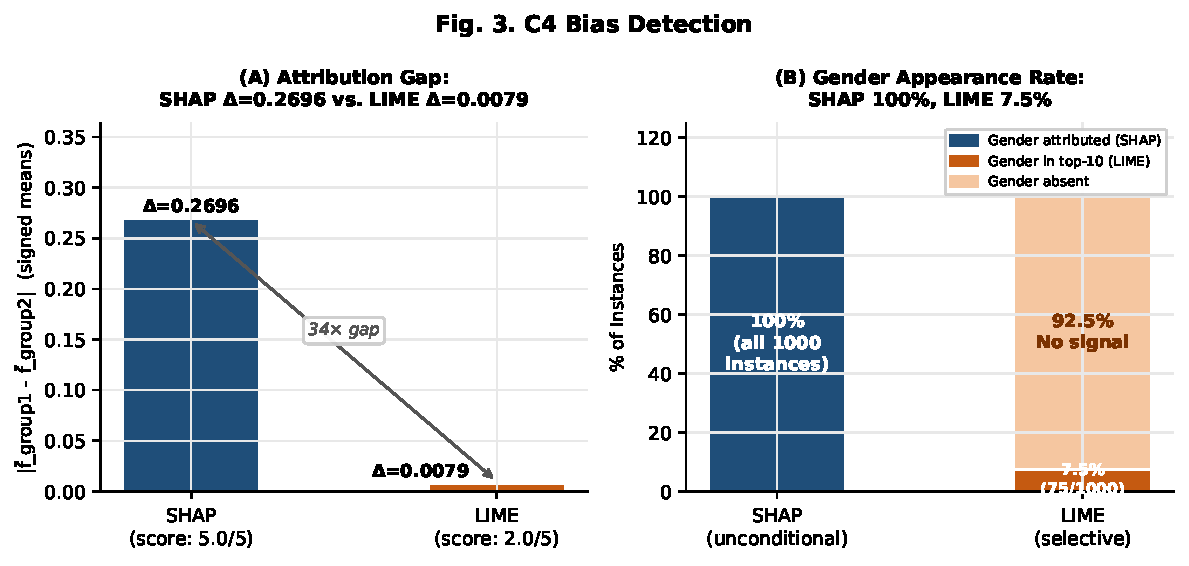
\includegraphics[width=\columnwidth]{fig3_bias_detection.pdf}
    \caption{C4 Bias Detection. (A) Attribution gap: SHAP $\Delta$=0.2696 vs. LIME $\Delta$=0.0079 (34$\times$). (B) Gender appearance rate: SHAP 100\% unconditional; LIME 7.5\%---gender absent from top-10 in 92.5\% of instances.}
    \label{fig:bias}
\end{figure}
\subsection{C5 --- Fairness Transparency}

The model produces a 21.6 pp approval rate disparity (73.9\% vs. 52.3\%). Both methods surface this at portfolio level; both score 5.0/5.0. Caveat: C5 measures a model property, not an XAI differentiator---a design limitation addressed in future revisions.

\subsection{C6 --- Human Oversight Support}

SHAP satisfies four Article~14(1) checklist dimensions: (i) decision direction clearly indicated by sign; (ii) quantitative influence magnitude; (iii) actionable feature-level information for corrective intervention; and (iv) full traceability from input to attribution. SHAP: $4.0/5.0$. LIME satisfies three of four dimensions---actionability is partially limited because condition-based explanations reference discretized ranges rather than continuous feature values, complicating precise intervention targeting. LIME: $3.5/5.0$.

\subsection{C7 --- Auditability}

SHAP is deterministic: any explanation regenerates
exactly from stored inputs and model weights alone. Score:
5.0/5.0. LIME's stochastic sampling requires per-instance seed
storage; fixed-seed LIME achieves $J = 1.000$ but shifts rather
than eliminates the compliance burden. Score: 2.0/5.0.

\subsection{Overall CSF Results}

\begin{table}[h]
\caption{CSF Compliance Scores: SHAP vs. LIME}
\label{tab:csf_scores}
\centering
\renewcommand{\arraystretch}{1.2}
\begin{tabular}{lcccc}
\toprule
\textbf{Criterion} & \textbf{Art.} & \textbf{SHAP} & \textbf{LIME} & \textbf{$\Delta$} \\
\midrule
C1: Coverage / Fidelity          & 13(1)    & 3.0 & 1.5 & +1.5 \\
C2: Consistency $\bigstar$       & 13(3)(b) & 5.0 & 1.0 & +4.0 \\
C3a: Structural Complexity       & 13(1)    & 4.0 & 1.0 & +3.0 \\
C3b: Comprehensibility $\blacktriangledown$ & 13(1) & 2.0 & 4.0 & $-$2.0 \\
C4: Bias Detection $\bigstar$    & 14(4)(b) & 5.0 & 2.0 & +3.0 \\
C5: Fairness Transparency        & 26(5)    & 5.0 & 5.0 & 0.0  \\
C6: Human Oversight              & 14(1)    & 4.0 & 3.5 & +0.5 \\
C7: Auditability                 & 13(3)    & 5.0 & 2.0 & +3.0 \\
\midrule
Overall (equal-weight mean)      & ---      & 4.12 & 2.50 & +1.62 \\
\bottomrule
\multicolumn{5}{p{8cm}}{\footnotesize $\bigstar$ Most consequential for Article compliance. $\blacktriangledown$ LIME advantage. Statistical test for C2: Mann-Whitney $U$=20,250,000, $p$$<$0.001 ($n$=4,500 pairwise Jaccard scores per method; $\binom{10}{2}$=45 run-pairs $\times$ 100 instances). Monte Carlo weight sensitivity ($n$=3,000 Dirichlet draws) confirms SHAP ranks higher in 99.0\% of configurations (robustness ratio = 0.9903). Equal-weight mean is a preliminary aggregation; institutions may weight criteria by their specific regulatory exposure.}
\end{tabular}
\end{table}

\begin{figure}[h]
    \centering
    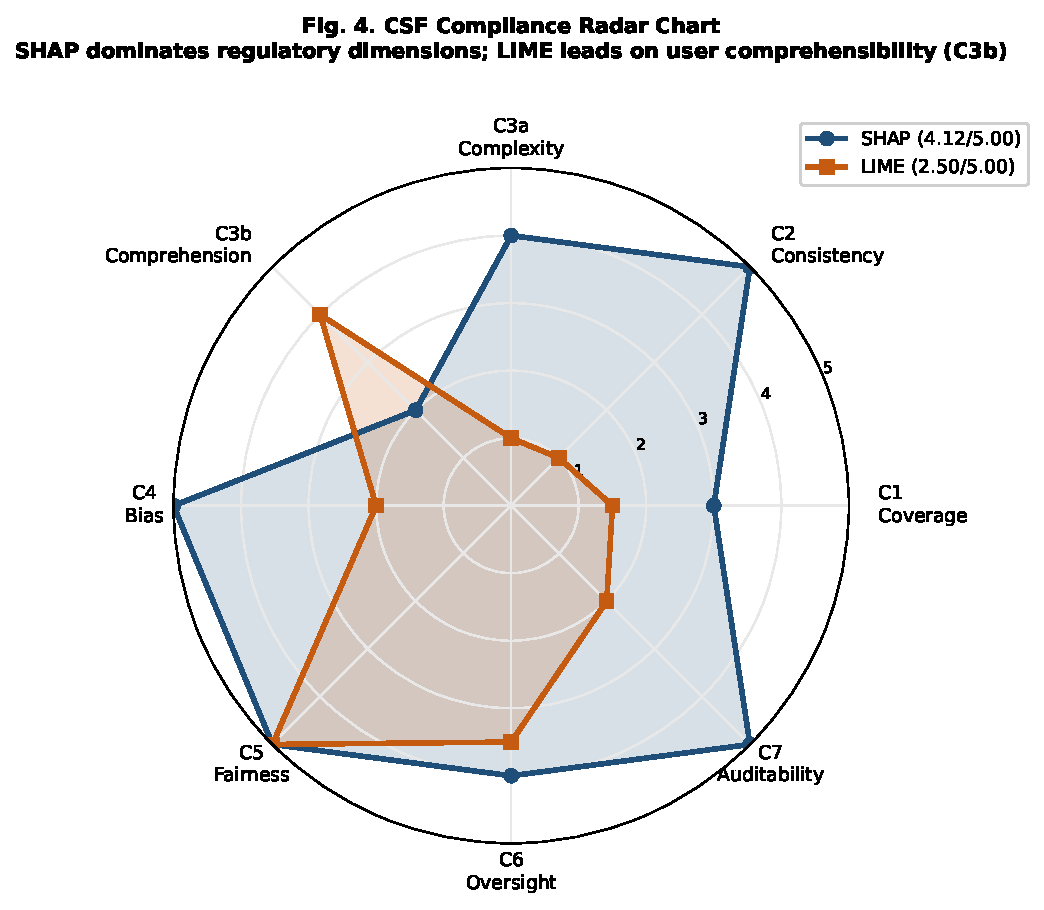
\includegraphics[width=\columnwidth]{fig4_radar_chart.pdf}
    \caption{Compliance radar chart across all seven CSF criteria (eight scores; C3 assessed on two sub-dimensions). SHAP (blue) dominates on regulatory dimensions; LIME (orange) leads only on user comprehensibility (C3b).}
    \label{fig:radar}
\end{figure}

\section{Discussion}

\subsection{Regulatory Profile of SHAP}

SHAP achieves $4.0$ or higher on six of seven criteria. Its mathematical determinism ($C_2$: $J = 1.000$) and unconditional attribution architecture ($C_4$: $100\%$ feature coverage) are inherent to the TreeSHAP algorithm---unreplicable by LIME regardless of configuration. SHAP explanations can be regenerated on demand from inputs alone; LIME explanations cannot.
\subsection{The Case for LIME in Customer-Facing Explainability}

LIME's C3b advantage (4.0 vs. 2.0) matters: Article 13(1) requires information comprehensible to deployers and affected persons; a condition-based explanation (`Debt Ratio $>$ 35\%: $-$0.25') is more accessible to non-experts than a raw Shapley magnitude, consistent with Kaur et al. \cite{b6}. We therefore recommend a hybrid deployment: SHAP for regulatory infrastructure, audit logs, and bias monitoring (Articles 13(3) and 14); LIME for customer-facing interfaces where semantic accessibility is primary (Article 13(1)), provided its fidelity is validated for the specific decisions being explained.


\subsection{Limitations and Validity Threats}

Seven limitations should be considered before applying the CSF.
(1)~\textit{Single dataset:} evaluation is conducted on a single publicly
available dataset with specific feature distributions, class imbalance, and
demographic composition; results should be validated on proprietary credit
datasets before institutional adoption.
(2)~\textit{Threshold calibration:} score conversion thresholds in Table~IV
are calibrated heuristically and may not reflect the exact enforcement
standards that EU AI Office implementation guidelines will
specify---guidelines not yet published as of this writing.
(3)~\textit{Qualitative criteria:} C3b, C6, and C7 scores reflect the
authors' structured assessments; inter-rater reliability studies with
independent evaluators are required before treating these scores as
definitive.
(4)~\textit{Legal interpretations:} the Article mappings represent the
authors' good-faith reading of statutory text; independent legal expert
review is required, particularly for C4's mapping to Article~14(4)(b).
(5)~\textit{C5 criterion design:} as currently operationalized, C5 measures
model-level fairness rather than a differentiating property of XAI methods;
future revisions should assess each method's ability to attribute the source
of approval disparities to specific algorithmic features.
(6)~\textit{Threshold sensitivity:} a formal ablation study of how CSF
scores change under threshold variations is identified as necessary future
work before the CSF is used as a definitive compliance instrument.
(7)~\textit{LIME configuration dependency:} the C1, C3a, and C4 scores were obtained with a specific LIME setup --- discretization on, $K=10$. As shown in Section~IV-A, those scores can look quite different under other configurations.

\subsection{Legal Uncertainty and Threshold Sensitivity}

The Act's qualified language---transparency ``to the extent necessary'' (Art. 13(1)); ``appropriate'' oversight (Art. 14(1))---will be concretized through EU AI Office guidelines and case law. Until then, any Article-to-metric mapping is interpretive rather than authoritative. Institutions should engage qualified legal counsel before treating CSF scores as definitive compliance indicators.

That said, the overall ranking is not hanging by a thread. The largest gaps between the two methods come from architectural facts --- SHAP's $J = 1.000$ will sit above any Score-5 threshold a reviewer might reasonably propose; LIME's $J = 0.381$ sits below Score-2 by a wide margin. The sensitive spot is C1: SHAP's coverage of 0.700 lands exactly at the Score-3 cut, so a shift in the band could move it down to a 2. Even so, the SHAP $>$ LIME ordering on C1 holds for threshold shifts up to $+16.7\%$, and LIME's $R^2$ of 0.251 is so far below its lowest scoring band (0.55) that no plausible recalibration would help it. C3a sits in a similar position and would benefit from a proper ablation study in future work.

\subsection{Robustness of CSF Rankings}

Two robustness tests confirm the SHAP-dominant ranking is not an artefact of equal-weight aggregation. First, a Monte Carlo analysis drew 3,000 Dirichlet(1) weight vectors over all eight criteria: SHAP ranked higher in 2,971/3,000 configurations (robustness ratio = 0.9903); the 29 LIME-favouring cases required C3b weight $> 0.6$. Second, a $\pm$10\% metric perturbation preserved the ranking in all cases (SHAP: 4.0--4.2; LIME: 2.1). The CSF conclusion is robust to both weighting assumptions and threshold calibration choices.

\begin{figure}[h]
    \centering
    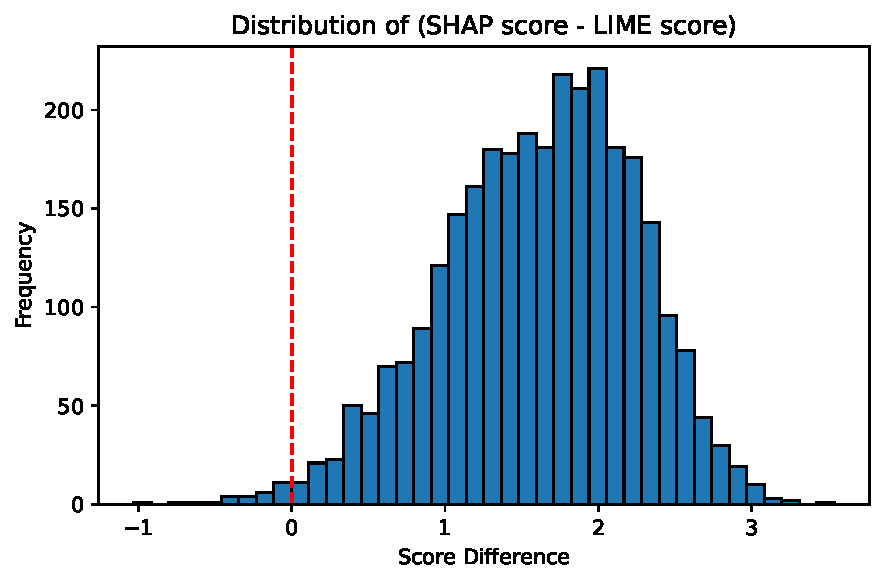
\includegraphics[width=\columnwidth]{fig_weight_sensitivity.pdf}
    \caption{Weight sensitivity analysis. Distribution of (SHAP score $-$ LIME score) across 3,000 randomly sampled weight vectors drawn from a Dirichlet(1) prior over all eight CSF criteria. The distribution lies almost entirely above zero (robustness ratio = 0.9903); negative differences occur only under extreme C3b over-weighting.}
    \label{fig:weight_sens}
\end{figure}

\subsection{Practical Deployment Considerations}

For bias monitoring (Article 14(4)(b)), institutions should not rely on LIME given its 92.5\% gender absence rate. SHAP's unconditional attribution architecture provides the consistent demographic signal required for Article 14 compliance dashboards.

Institutions should recalibrate Table~\ref{tab:score_thresh}'s thresholds as EU AI Office guidance emerges, particularly for C1 and C2.

\section{Conclusion}

This paper presents the Compliance Scoring Framework—to our knowledge, this is the first framework to operationalize selected requirements of EU AI Act Articles 13, 14, and 26 as measurable and reproducible criteria for evaluating XAI methods. Applied to SHAP and LIME on 307,511 real credit applica- tions, SHAP achieves superior overall compliance (4.12/5.00 vs. 2.50/5.00). The primary differentiators—explanation con- sistency ($J = 1.000$ vs. $0.381$, $p < 0.001$), bias detection sensitivity (gender present in 100\% of SHAP explanations vs. absent from LIME's top-10 in 92.5\% of instances), and auditability—reflect fundamental architectural differences that persist across parameter config- urations. A kernel width sweep confirms LIME’s low fidelity is structural. LIME’s advantage in user comprehensibility motivates a hybrid deployment strategy: SHAP for regulatory infrastructure, LIME for customer-facing interfaces.

The CSF provides financial institutions with an action- able evaluation tool ahead of the August 2026 enforcement deadline. Future work should validate the CSF on multiple credit datasets, run controlled comprehension studies with non-expert users, and seek independent legal review of the Article mappings as EU AI Office guidance emerges. The framework is extensible to additional XAI methods in- cluding counterfactual explanations~\cite{b13}.

\begin{thebibliography}{00}

% [1] — first cited in Introduction
\bibitem{b2}
European Parliament and Council, ``Regulation (EU) 2024/1689 of the European Parliament and of the Council (EU Artificial Intelligence Act),'' \textit{Official Journal of the European Union}, Jul. 2024.

% [2] — first cited in Introduction
\bibitem{b3}
P. Hacker and M. Eber, ``The future of credit underwriting and insurance under the EU AI Act,'' \textit{Harvard Data Science Review}, Issue 7.3, 2025.

% [3] — first cited in Introduction
\bibitem{b4}
S. M. Lundberg and S.-I. Lee, ``A unified approach to interpreting model predictions,'' in \textit{Advances in Neural Information Processing Systems (NIPS)}, vol. 30, 2017, pp. 4765--4774.

% [4] — first cited in Introduction
\bibitem{b5}
M. T. Ribeiro, S. Singh, and C. Guestrin, ``Why should I trust you?: Explaining the predictions of any classifier,'' in \textit{Proc. 22nd ACM SIGKDD Int. Conf. Knowledge Discovery and Data Mining}, 2016, pp. 1135--1144.

% [5] — first cited in Introduction
\bibitem{b8}
R. Guidotti et al., ``A survey of methods for explaining black box models,'' \textit{ACM Computing Surveys}, vol. 51, no. 5, 2018.

% [6] — first cited in Introduction
\bibitem{b9}
M. Nauta et al., ``From anecdotal evidence to quantitative evaluation: A systematic review on evaluating explainability,'' \textit{ACM Computing Surveys}, vol. 55, no. 13s, 2023.

% [7] — first cited in Related Work
\bibitem{b11}
S. M. Lundberg et al., ``From local to global understanding with explainable AI for trees,'' \textit{Nature Machine Intelligence}, vol. 2, no. 1, pp. 56--67, 2020.

% [8] — first cited in Related Work
\bibitem{b15}
A. Gramegna and P. Giudici, ``SHAP and LIME: An evaluation of discriminative power in credit risk,'' \textit{Frontiers in Artificial Intelligence}, vol. 4, p. 752558, 2021.

% [9] — first cited in Related Work
\bibitem{b6}
H. Kaur et al., ``Interpreting interpretability: Understanding data scientists' use of interpretability tools for ML,'' in \textit{Proc. CHI Conf. Human Factors in Computing Systems}, 2020.

% [10] — first cited in Related Work
\bibitem{b14}
D. Alvarez-Melis and T. S. Jaakkola, ``On the robustness of interpretability methods,'' in \textit{ICML Workshop on Human Interpretability in Machine Learning (WHI)}, 2018.

% [11] — first cited in Related Work
\bibitem{b7}
C. Panigutti et al., ``The role of explainable AI in the context of the AI Act,'' in \textit{Proc. ACM FAccT}, 2023, pp. 1139--1150.

% [12] — first cited in Methodology
\bibitem{b10}
Home Credit Group, ``Home Credit Default Risk,'' Kaggle Dataset, 2018. [Online]. Available: https://www.kaggle.com/c/home-credit-default-risk

% [13] — first cited in Methodology
\bibitem{b1}
G. Ke et al., ``LightGBM: A highly efficient gradient boosting decision tree,'' in \textit{Advances in Neural Information Processing Systems (NIPS)}, vol. 30, 2017, pp. 3146--3154.

% [14] — first cited in Methodology
\bibitem{b12}
T. Miller, ``Explanation in artificial intelligence: Insights from the social sciences,'' \textit{Artificial Intelligence}, vol. 267, pp. 1--38, 2019.

% [15] — first cited in Results
\bibitem{b16}
D. Slack et al., ``Fooling LIME and SHAP: Adversarial attacks on post hoc explanation methods,'' in \textit{Proc. AIES}, 2020, pp. 180--186.

% [16] — first cited in Conclusion
\bibitem{b13}
S. Wachter, B. Mittelstadt, and C. Russell, ``Counterfactual explanations without opening the black box,'' \textit{Harvard J. Law \& Technology}, vol. 31, 2018.

\end{thebibliography}

\end{document}
